\documentclass[]{article}
\usepackage[a4paper, total={15cm,23cm}]{geometry}
\usepackage{fancyhdr}
\usepackage{graphicx}
\usepackage{amsmath}
\usepackage{amssymb}
\usepackage[dvipsnames]{xcolor}
\usepackage{tikz}
\usepackage{verbatim}
\usepackage{tcolorbox}
\usepackage{textcomp}
\usepackage{xcomment}
\usepackage{xstring}
%opening
\title{PH 223 Week 10}
\author{Benjamin Bauml and Danielle Skinner}
\date{Winter 2024}
\pagestyle{fancy}
\rhead{PH 223}
\chead{Winter 2024}
\lhead{Week 10}

% Version 2024-02-21
% Changes
% 2024-02-21 Added xstring package to enable smooth implementation of new \ModePage command.
% For Assignment, leave Purpose as 1. For Worksheet, set to 2. For Student Solution, set to 3. For Teacher Solution, set to 4.
\newcommand{\Purpose}{1}

\newcommand{\Exclusion}{0}
\newcommand{\PageTurn}{0}
\newcommand{\GrayProb}{0}
\newcommand{\Tipsy}{0}

% Assignment
\if\Purpose1
\renewcommand{\Exclusion}{1}
\fi
% Worksheet
\if\Purpose2
\renewcommand{\Exclusion}{1}
\renewcommand{\PageTurn}{1}
\fi
% Student Solution
\if\Purpose3
\renewcommand{\PageTurn}{1}
\renewcommand{\GrayProb}{1}
\fi
% Teaching Copy
\if\Purpose4
\renewcommand{\PageTurn}{1}
\renewcommand{\GrayProb}{1}
\renewcommand{\Tipsy}{1}
\fi

\if\Exclusion1
\xcomment{Title,Problem,ProblemSub,PassFig}
\fi

\def \NewQ {0}
\def \PForce {0}
\newcommand{\MaybePage}[1]{
	\def \PForce {#1}
	\if\PForce1
		\newpage
	\else
		\if\NewQ0
		\gdef \NewQ {\PageTurn}
		\else
		\newpage
		\fi
	\fi
}

\newcommand{\ModePage}[1]{
	\IfSubStr{#1}{\Purpose}{\newpage}{}
}

\newenvironment{Problem}[2][0]{%The first argument is optional, and if it is set to 1, the \newpage will be forced.
\MaybePage{#1}
\section*{#2}
\if\GrayProb1
\begin{tcolorbox}[colback=lightgray,colframe=lightgray,sharp corners,boxsep=1pt,left=0pt,right=0pt,top=0pt,bottom=0pt,after skip=2pt]
\else
\begin{tcolorbox}[colback=white,colframe=white,sharp corners,boxsep=1pt,left=0pt,right=0pt,top=0pt,bottom=0pt,after skip=2pt]
\fi
}{
\end{tcolorbox}\noindent
}

\newenvironment{ProblemSub}[1][0]{%The argument is optional, and if a string of numbers is entered into it, it will force a \newpage in any \Purpose that shows up in the string. For example, "13" would lead to the newpage being forced in modes 1 and 3.
\ModePage{#1}
\if\GrayProb1
\begin{tcolorbox}[colback=lightgray,colframe=lightgray,sharp corners,boxsep=1pt,left=0pt,right=0pt,top=0pt,bottom=0pt,after skip=2pt]
\else
\begin{tcolorbox}[colback=white,colframe=white,sharp corners,boxsep=1pt,left=0pt,right=0pt,top=0pt,bottom=0pt,after skip=2pt]
\fi
}{
\end{tcolorbox}\noindent
}

\newenvironment{PassFig}{\begin{figure}[h]}{\end{figure}}

\newcommand{\TeachingTips}[1]{
\if\Tipsy1
\begin{tcolorbox}[colback=lightgray,colframe=black]
#1
\end{tcolorbox}
\fi
}

\newenvironment{Title}{\maketitle}{}

\begin{document}
\begin{Title}
\begin{center}
	The last two problems are borrowed/adapted from Chapters 29 and 30 of the \textit{Student Workbook} for \textit{Physics for Scientists and Engineers}. The first problem is from the Week 9 Help and Practice Problems for PH 213, and probably was originally sourced from the same textbook.
\end{center}
\end{Title}

\begin{Problem}{Activity 1}
	Use the Biot-Savart law to find the magnetic field strength at the center of the semicircle in the figure below.
\end{Problem}
\begin{PassFig}
	\centering
	%\includegraphics[scale=0.5]{curved_wire.png}
	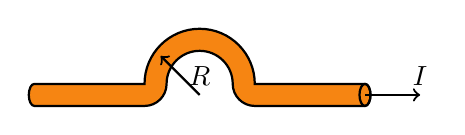
\begin{tikzpicture}[scale=0.7]
		\filldraw[thick,color=black,fill=BurntOrange] (-1,0.2) arc (180:0:1) -- (3,0.2) arc (90:-90:0.1 and 0.2) -- (1,-0.2) arc (270:180:0.4) arc (0:180:0.6) arc (0:-90:0.4) -- (-3,-0.2) arc (270:90:0.1 and 0.2) -- cycle;
		\draw[thick] (3,0) ellipse (0.1cm and 0.2cm);
		\draw[thick,->] (0,0) -- ({cos(135)},{sin(135)});
		\node[anchor=south] at (0,0) {$R$};
		\draw[thick,->] (3,0) -- (4,0);
		\node[anchor=south] at (4,0) {$I$};
	\end{tikzpicture}
\end{PassFig}

We will tackle this problem using the Chop-Multiply-Add method.
The Biot-Savart law is:
\[
	\vec{B} = \frac{\mu_o}{4\pi}\frac{q\vec{v}\times\hat{r}}{r^2}	
\]

Let's first consider the magnetic field due to the two straight sides. The current moves in the $+\hat{x}$ direction, and the $\hat{r}$ is in the $\pm\hat{x}$. Therefore the cross-product in the Biot-Savart law is zero. The straight sides don't contribute a magnetic field to the center of the loop. So we only need to focus on the curved portion!

\begin{figure}[h]
	\centering
	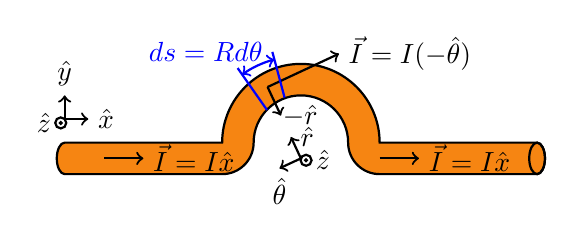
\begin{tikzpicture}
		\filldraw[thick,color=black,fill=BurntOrange] (-1,0.2) arc (180:0:1) -- (3,0.2) arc (90:-90:0.1 and 0.2) -- (1,-0.2) arc (270:180:0.4) arc (0:180:0.6) arc (0:-90:0.4) -- (-3,-0.2) arc (270:90:0.1 and 0.2) -- cycle;
		\draw[thick] (3,0) ellipse (0.1cm and 0.2cm);
		\draw[thick,->] (0,0) -- ({0.3*cos(115)},{0.3*sin(115)});
		\node[anchor=west] at ({0.3*cos(115)},{0.3*sin(115)}) {$\hat{r}$};
		\draw[thick,->] (0,0) -- ({-0.3*sin(115)},{0.3*cos(115)});
		\node[anchor=north] at ({-0.3*sin(115)},{0.3*cos(115)}) {$\hat{\theta}$};
		\filldraw ({-0.07*cos(160)},{-0.07*sin(160)}) circle (0.02);
		\draw[thick] ({-0.07*cos(160)},{-0.07*sin(160)}) circle (0.07);
		\node[anchor=west] at ({-0.07*cos(160)},{-0.07*sin(160)}) {$\hat{z}$};
		\draw[thick,->] ({cos(115)},{sin(115)}) -- ({cos(115)+1*sin(115)},{sin(115)-1*cos(115)});
		\node[anchor=west] at ({cos(115)+1*sin(115)},{sin(115)-1*cos(115)}) {$\vec{I} = I(-\hat{\theta})$};
		\draw[thick,->] ({cos(115)},{sin(115)}) -- ({cos(115)-0.4*cos(115)},{sin(115)-0.4*sin(115)});
		\node[anchor=west] at ({cos(115)-0.4*cos(115)-0.1},{sin(115)-0.4*sin(115)}) {$-\hat{r}$};
		\begin{scope}[rotate=-55]
			\draw[thick,blue] (-0.75,0) -- (-1.4,0);
		\end{scope}
		\begin{scope}[rotate=-75]
			\draw[thick,blue] (-0.8,0) -- (-1.4,0);
		\end{scope}
		\begin{scope}[rotate=-55]
			\draw[thick,blue,<->] (-1.3,0) arc (180:160:1.3);
		\end{scope}
		\node[anchor=east] at ({-1.4*cos(75)},{1.4*sin(75)}) {\color{blue}$ds = Rd\theta$};
		\begin{scope}[shift={(-2.5,0)}]
			\draw[thick,->] (0,0) -- (0.5,0);
			\node[anchor=west] at (0.5,0) {$\vec{I}=I\hat{x}$};
		\end{scope}
		\begin{scope}[shift={(1,0)}]
			\draw[thick,->] (0,0) -- (0.5,0);
			\node[anchor=west] at (0.5,0) {$\vec{I}=I\hat{x}$};
		\end{scope}
		\begin{scope}[shift={(-3,0.5)}]
			\draw[thick,->] (0,0) -- (0.3,0);
			\node[anchor=west] at (0.3,0) {$\hat{x}$};
			\draw[thick,->] (0,0) -- (0,0.3);
			\node[anchor=south] at (0,0.3) {$\hat{y}$};
			\filldraw ({-0.07*cos(45)},{-0.07*sin(45)}) circle (0.02);
			\draw[thick] ({-0.07*cos(45)},{-0.07*sin(45)}) circle (0.07);
			\node[anchor=east] at ({-0.07*cos(45)},{-0.07*sin(45)}) {$\hat{z}$};
		\end{scope}
	\end{tikzpicture}
\end{figure}

Starting with the ``Chop" part, we can rewrite the cross product:
\[
	dq\vec{v}\times\hat{r} = ds\vec{I}\times\hat{r} = (Rd\theta)I(-\hat{\theta}) \times (-\hat{r}) = IRd\theta (-\hat{z}).
\]
To do this calculation, we switched to a cylindrical coordinate system. The current moves in the $-\hat{\theta}$ direction, and the $\hat{r}$ points from the wire to the center of the semi-circle, making it negative.

\TeachingTips{
\[
dq\cdot v = dq\cdot\frac{ds}{dt} = ds\cdot\frac{dq}{dt} = ds\cdot I 
\]
}

Now on to ``Multiply.'' The infinitesimal magnetic field can now be written as
\[
	d\vec{B} = \frac{\mu_o}{4\pi}\frac{dq\vec{v}\times\hat{r}}{r^2} = \frac{\mu_o}{4\pi}\frac{IRd\theta}{R^2} (-\hat{z}).
\]
Finally, the ``Add'':
\[
	\vec{B} = \frac{\mu_o}{4\pi}\frac{I}{R}(-\hat{z})\int_{0}^{\pi} d\theta.
\]
The final answer is therefore
\[
	\vec{B} = \frac{\mu_o}{4}\frac{I}{R}(-\hat{z}).
\]
We can see that this is half the result of a magnetic field due to a current loop!

\begin{Problem}{Activity 2}
	The capacitor in this circuit was initially charged, then the switch was closed. At this instant of time, the potential difference across the resistor is $ \Delta V_{R} = 4 $ V.
\end{Problem}
\begin{PassFig}
	\centering
	\includegraphics[scale=1.2]{RC}
\end{PassFig}
\begin{ProblemSub}
	(a) At this instant of time, what is the current through the resistor? %What is the current through the space between the capacitor plates?
\end{ProblemSub}
The current through the resistor at the instant the switch closes is
\[
	I_{0} = \frac{\Delta V_{R}}{R} = \frac{4\text{ V}}{2\text{ \textohm}} = 2\text{ A}.
\]
%No charge actually crosses the gap between the plates, so $ I_{through} = 0 $ A.
\begin{ProblemSub}
	(b) What is the current through the resistor over time?
\end{ProblemSub}
A discharging RC circuit has current of the form
\[
	I(t) = I_{0} e^{-t/\tau}.
\]
We just found $ I_{0} $, and for the given circuit, $ \tau = RC = (2\text{ \textohm})(\frac{1}{2}\text{ F}) = 1 $ s. As such,
\[
	I(t) = (2\text{ A}) e^{-t/(1\text{ s})}.
\]
\begin{ProblemSub}
	(c) What is the charge in the capacitor over time?
\end{ProblemSub}
A discharging RC circuit has charge of the form
\[
	Q(t) = Q_{0}e^{-t/\tau}.
\]
The initial charge $ Q_{0} = \Delta V_{C} C $, and the initial voltage difference across the capacitor must be $ \Delta V_{C} = 4 $ V by Kirchhoff's loop law. As such, $ Q_{0} = (4\text{ V})(\frac{1}{2}\text{ F}) = 2\text{ C} $, and the charge varies over time as
\[
	Q(t) = (2\text{ C})e^{-t/(1\text{ s})}.
\]
\begin{ProblemSub}
(d) If the capacitor consists of two parallel plates of area $ A $, symbolically calculate the electric flux between them, and the time derivative of this flux. %Use this to obtain the displacement current.
\end{ProblemSub}
Assuming uniform distribution of charge over the plate, the surface charge density across the positive side is
\[
	\sigma(t) = \frac{Q(t)}{A} = \frac{Q_{0}}{A}e^{-t/\tau}.
\]
Thus, the electric field magnitude between the plates is
\[
	E = \frac{\sigma(t)}{\epsilon_{0}} = \frac{Q_{0}}{A\epsilon_{0}}e^{-t/\tau}.
\]
As such, the flux through the cross-sectional area $ A $ of the region between the plates is
\[
	\Phi_{e} = EA = \frac{Q_{0}}{\epsilon_{0}}e^{-t/\tau}.
\]
	This flux changes in time as
\[
	\frac{d\Phi_{e}}{dt} = -\frac{Q_{0}}{\tau\epsilon_{0}}e^{-t/\tau} = -\frac{Q_{0}}{RC\epsilon_{0}}e^{-t/\tau} = -\frac{\Delta V_{R}}{R\epsilon_{0}}e^{-t/\tau} = -\frac{I_{0}}{\epsilon_{0}}e^{-t/\tau}.
\]
\begin{comment}
Displacement current is defined to be $ I_{disp} = \epsilon_{0}\frac{d\Phi_{e}}{dt} $, so
\[
	I_{disp}(t) = -I_{0}e^{-t/\tau} = -I(t).
\]
We see that the magnitude of displacement current is the same as the magnitude of true current in the system over time. The negative sign indicates that the displacement current is opposite the electric field in the capacitor (caused by the field decreasing). This would make the current flow toward the positive plate, and actual current is leaving this plate down the wire as the capacitor discharges, so the direction of the displacement current is actually consistent with the direction of true current in the system.
\end{comment}

\begin{Problem}{Activity 3}
	The capacitor in an $ LC $ circuit has maximum charge at $ t = 1 $ \textmu s. The current through the inductor next reaches a maximum at $ t = 3 $ \textmu s.
\end{Problem}
\begin{ProblemSub}
	(a) When will the inductor current reach a maximum in the opposite direction?
\end{ProblemSub}
The current in an $ LC $ circuit oscillates as $ I = I_{max}\sin(\omega t + \phi) $, where $ \phi $ is some phase constant. The charge on the capacitor is maximum when the current is zero, so the two events are 90$ ^{\circ} $ out of phase. That means the time between the two is a quarter of the circuit's period:
\[
\Delta t = 2\text{ \textmu s} = \frac{T}{4}.
\]
The inductor current changes direction after a 180$ ^{\circ} $ phase change, so we need to add half of the period ($ T/2 = 4 $ \textmu s) to the time of the first maximum ($ t = 3 $ \textmu s) to reach the inverted maximum. That gives us the desired time of $ t = 7 $ \textmu s.
\begin{ProblemSub}
	(b) What is the circuit's period of oscillation?
\end{ProblemSub}
As we said before, $ \Delta t = \frac{T}{4} $, so $ T = 8 $ \textmu s.
\end{document}
